\documentclass[a4paper]{article}

\usepackage[czech]{babel}
\usepackage[utf8x]{inputenc}
\usepackage[T1]{fontenc}
\usepackage{amsmath}
\usepackage{graphicx}
\usepackage[left=2cm,text={17cm, 25.7cm},top=2cm]{geometry}

\title{\textbf{1. samostatná práce\\IMA\\Zadání 9}}
\author{Adam Šulc - xsulca00\\ Tomáš Ulický - xulick01\\ Daniel Rudík - xrudik00\\ Ondrej Svoreň - xsvore01\\ Adrián Tomašov - xtomas32\\ Jozef Urbanovský - xurban66}
\date{}

\begin{document}
	\maketitle
	\begin{center}
	
\includegraphics[clip]{FIT.png}
	\end{center}
	\newpage
	\section*{1. príklad}
	
	Rozložte na parciální zlomky racionální lomenou funkci 
	\begin{align*}
	f(x)= \dfrac{9x^3+33x^2+17x-23} {x^5+7x^4+16x^3+16x^2+15x+9}
	\end{align*}
	Použijeme Hornerovo schéma pre rozklad polynómu na súčinový tvar \\ \\
	\begin{align*}
	\begin{array}{c|cccccc}
	HS & 1 & 7 & 16 & 16 & 15 & 9 \\ \hline
	-1 & 1 & 6 & 10 & 6  & 9  & 0 \\ 
	-3 & 1 & 3 & 1  & 3  & 0      \\ 
	-3 & 1 & 0 & 1 & 0            \\ \hline
	\end{array}
	\end{align*}
	
	\begin{align*}
	(x+1)(x^4+6x^3+10x^2&+6x+9) \\
	(x+1)(x+3)(x^3+3x^2&+x+3)   \\
	(x+1)(x+3)^2(x^2+1)&
	\end{align*}
	
	\begin{align*}
	\dfrac{9x^3+33x^2+17x-23} {(x+1)(x+3)^2(x^2+1)} = 
	\dfrac{A}{x+1} & + \dfrac{B}{x+3} + \dfrac{C}{(x+3)^2} + \dfrac{Dx+E}{x^2+1}\\
	\\
	9x^3+33x^2+17x-23 = 
	A(x+3)^2(x^2+1) + B(x+1)(x&+3)(x^2+1) + C(x+1)(x^2+1) + Dx+E(x+1)(x+3)^2
	\end{align*}

	\begin{align*}
	\text{Keď dosadíme prvý koreň rovnice -1, následne } A = -2\\
	\text{Keď dosadíme druhý koreň rovnice -3, následne } C = 1
	\end{align*}
	

	Keď dosadíme vypočítané hodnoty premenných získame: 
	\\
	
	$9x^3 + 33x^2 + 17x - 23 = (-2)(x+3)^2(x^2 + 1) + B(x+1)(x+3)(x^2+1) +
	1(x+1)(x^2+1) + (D + Ex)(x+1)(x+3)^2$
	\\
	
	Roznásobíme:
	\\
	
	$9x^3 + 33x^2 + 17x - 23 = Bx^4 + Ex^4 + 4Bx^3 + 7Ex^3 + Dx^3 + 4Bx^2 +
	15Ex^2 + 7Dx^2 + 4Bx + 15Dx + 9Ex - 2x^4 - 11x^3 - 19x^2 - 11x + 3B + 9D - 17$
	\\
	
	Zoskupíme prvky podľa premennej x a zostavíme maticu:
	\\
	
	$9x^3 + 33x^2 + 17x - 23 = x^4(-2 + B + E) + x^3(4B + 7E - 11 + D) + 
	x^2(4B + 7D + 15E - 19) + x(4B + 9E + 15D - 11) + (3B + 9D - 17)$
	
	\\
	\begin{center}$
	\begin{bmatrix}
		3a_1+9a_3-17=-23\\
		4a_1+15a_3+9a_4-11=17\\
		4a_1+15a_4+7a_3-19=33\\
		4a_1+7a_4+a_3-11=9\\
		a_1+a_4-2=0
	\end{bmatrix}$
	\end{center}
	\begin{align*}
	A&=-2\\
	B&=-2\\
	C&=1\\
	D&=0\\
	E&=4
	\end{align*}
	
	\begin{align*}
	\dfrac{-2}{x+1} & + \dfrac{-2}{x+3} + \dfrac{1}{(x+3)^2} + \dfrac{4x+0}{x^2+1} =\\
	\dfrac{4x}{x^2+1} & - \dfrac{2}{x+1} - \dfrac{2}{x+3} + \dfrac{1}{(x+3)^2}
	\end{align*}
	
	\newpage
	
	\section*{2. príklad}
	
	
	Najděte asymptoty grafu funkce. $f(x) = \dfrac{x \sqrt{x^2+1}}{2x^2-1}$
	
	\begin{center}
	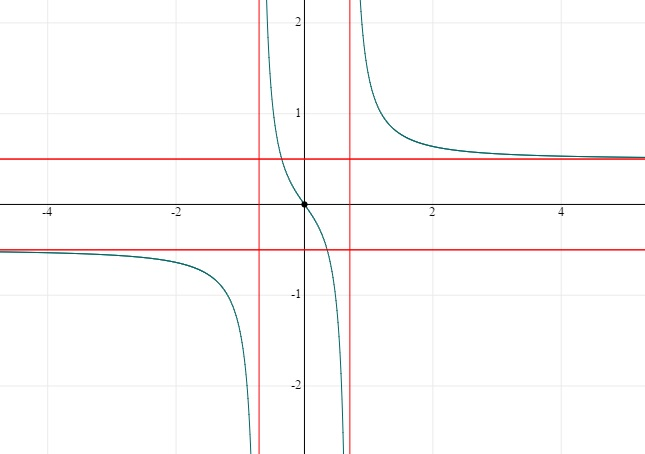
\includegraphics[width=11cm]{dvojka.jpg}
	\end{center}
	\begin{align*}
	f(x) & = \dfrac{x \sqrt{x^2+1}}{2x^2-1}\\
	2x^2 & = 1\\
	x^2 & = \dfrac{1}{2}\\
	x & = \pm\sqrt{\dfrac{1}{2}}\\
	D(f) & = \mathbb{R} -\{\ \pm \dfrac{1}{\sqrt{2}} \} \\
	\end{align*}
	Prejdeme nedefinové body funkcie a overíme, či nespĺňajú aj podmienku asymptót bez smernice, pre ktoré má platiť nasledovné: 
	\[ \lim_{x \to a^+} = \pm \infty \qquad \lim_{x \to a^-} = \pm \infty\]
	Využijeme nasledovné pravidlá nevlastných limít (\textit{k} označuje ľubovoľné kladné reálne číslo).
	\[ \dfrac{k}{0^+}= \infty \qquad \dfrac{k}{0^-} = -\infty\]
	
	\[ \lim_{x \to {\frac{1}{\sqrt 2}}^+}  \dfrac{x \sqrt{x^2+1}}{2x^2-1} = 
	\lim_{x \to {\frac{1}{\sqrt 2}}^+}  \dfrac{\frac{1}{\sqrt 2} \sqrt{(\frac{1}{\sqrt 2})^2+1}}{2(\frac{1}{\sqrt 2})^2-1} =
	\lim_{x \to {\frac{1}{\sqrt 2}}^+}  \dfrac{\frac{1}{\sqrt 2} \sqrt{\frac{3}{2}}}{0^+} = \infty \]\\
	
	\[ \lim_{x \to {\frac{1}{\sqrt 2}}^-}  \dfrac{x \sqrt{x^2+1}}{2x^2-1} = 
	\lim_{x \to {\frac{1}{\sqrt 2}}^-}  \dfrac{\frac{1}{\sqrt 2} \sqrt{(\frac{1}{\sqrt 2})^2+1}}{2(\frac{1}{\sqrt 2})^2-1} =
	\lim_{x \to {\frac{1}{\sqrt 2}}^-}  \dfrac{\frac{1}{\sqrt 2} \sqrt{\frac{3}{2}}}{0^-} = -\infty \]\\
	
	\[ \lim_{x \to {-\frac{1}{\sqrt 2}}^+}  \dfrac{x \sqrt{x^2+1}}{2x^2-1} = 
	\lim_{x \to {-\frac{1}{\sqrt 2}}^+}  \dfrac{-\frac{1}{\sqrt 2} \sqrt{(-\frac{1}{\sqrt 2})^2+1}}{2(-\frac{1}{\sqrt 2})^2-1} =
	\lim_{x \to {-\frac{1}{\sqrt 2}}^+}  \dfrac{-\frac{1}{\sqrt 2} \sqrt{\frac{3}{2}}}{0^+} = \infty \]\\
	
	
	\[ \lim_{x \to {-\frac{1}{\sqrt 2}}^-}  \dfrac{x \sqrt{x^2+1}}{2x^2-1} = 
	\lim_{x \to {-\frac{1}{\sqrt 2}}^-}  \dfrac{-\frac{1}{\sqrt 2} \sqrt{(-\frac{1}{\sqrt 2})^2+1}}{2(-\frac{1}{\sqrt 2})^2-1} =
	\lim_{x \to {-\frac{1}{\sqrt 2}}^-}  \dfrac{-\frac{1}{\sqrt 2} \sqrt{\frac{3}{2}}}{0^-} = -\infty \]\\
	
	\begin{center}
	Týmto sme dokázali, že bod podozrivý z extrémizmu je zároveň aj asymptotou danej funkcie.
	Následne sa pokúsime nájsť asymptoty so smernicou, využijeme vzťah \[a=\lim \dfrac{f(x)}{x}\]
	\end{center}
	
	\[ \lim_{x \to \infty}  \dfrac{\dfrac{x \sqrt{x^2+1}}{2x^2-1}}{x} = \\
	\lim_{x \to \infty}  \dfrac{|x| \sqrt{1+\dfrac{1}{x^2}}}{x^2(2-\dfrac{1}{x^2})} = \\
	\dfrac{1}{2} \lim_{x \to \infty} \dfrac{|x|}{x^2} = \]\\
	
	\[ \dfrac{1}{2}\lim_{x \to +\infty} \dfrac{x}{x^2} = 0 \qquad \dfrac{1}{2}\lim_{x \to -\infty} \dfrac{-x}{x^2} = 0\] \\
	
	\begin{center}
	Výsledkom danej limity je 0, to znamená, že asymptota nemá smernicu. V predpise y = 0x + q.
	To znamená, že nemá smernicu, teda asymptota bude vodorovná s osou x a graf funkcie sa k nej blíži v $\pm\infty$\\
	Musí platiť : 
	\[ \lim_{x \to \pm \infty} f(x)= a \in \mathbb{R} \qquad resp. \qquad \lim_{x \to \pm \infty} f(x)= b \in \mathbb{R} \] 
	\end{center}
	\[ \lim_{x \to \pm \infty}  \dfrac{x \sqrt{x^2+1}}{2x^2-1} = \lim_{x \to \pm \infty} \dfrac{x^2 \sqrt{1+\dfrac{1}{x^2}}}{x^2(2-\dfrac{1}{x^2})} = \dfrac{1}{2}\lim_{x \to \pm\infty} \dfrac{|x|}{x}  \]\\
	
	\[ \dfrac{1}{2}\lim_{x \to +\infty} \dfrac{x}{x} = \dfrac{1}{2} \qquad \dfrac{1}{2}\lim_{x \to -\infty} \dfrac{-x}{x} = -\dfrac{1}{2}\] \\
	
	$$x_1 = \underline{\dfrac{1}{\sqrt{2}}} \qquad x_2 = \underline{-\dfrac{1}{\sqrt{2}}} $$\\
	$$y_1 = \underline{\dfrac{1}{2}} \qquad y_2 = \underline{-\dfrac{1}{2}} $$
	\newpage
	
	\section*{3. príklad}
	 Knihkupectví získalo určitou knihu od vydavatele jako dar za 3 dolary za kus a prodává ji za cenu 15 dolarů za kus.
	 Při této ceně se prodalo 200 knih za měsíc. Aby se stimuloval prodej, chce knihkupectví cenu snížit a odhaduje,
	 že za každý 1 dolar snížené ceny se prodá měsíčně o 20 knih více. Určete, při jaké ceně knihy dosáhne knihkupectví
	 největší zisk z jejího prodeje. \\
	15\,\$...\hspace{3cm}200\,ks\\
	14\,\$...\hspace{3cm}220\,ks\\
	4\,\$...\hspace{3.17cm}420\,ks\\
	x\,\$...\hspace{3.17cm}(200+20(15-x))\,ks\\ \rule{6cm}{0.4pt}\\
	x...\hspace{3.37cm}cena 1 knihy\\
	x - 3...\hspace{2.83cm}zisk za 1 knihu\\
	(500-20x)...\hspace{2.09cm}počet predaných kníh\\
	Z toho predpis funkcie:
	
	\begin{align*}
	f(x) & =  (x - 3)(500 - 20x)\\
	f(x) & =  500x - 20x^2 - 1500 + 60x
	\intertext{Pričom funkčná hodnota vyjadruje zisk za mesiac pri cene x. Pomocou derivácie nájdeme bod, v ktorom má funkcia extrém.}
	f'(x) & =  500 - 40x + 60\\
	f'(x) & =  560 - 40x\\
	f'(x) & =  40(14 - x)\\
	\\
	f'(x) & = 0\\
	40(14 - x) & = 0\\
	14 - x & = 0\\
	x & = 14
	\intertext{Následne prešetríme monotónnosť funkcie a teda dosadíme hodnoty z intervalu $\left( -\infty,14\right)$ a $\left( 14,\infty\right)$.}
	x & = 13\\
	40(14 - x) & = ?\\
	40(14 - 13) & = 40\\
	f(x)' & > 0\\
	\intertext{Funkcia je na intervale $\left( -\infty,14\right)$ rastúca.}
	x & = 15\\
	40(14 - x) & = ?\\
	40(14 - 15) & = -40\\
	f(x)' & < 0\\
	\intertext{Funkcia je na intervale $\left( 14,\infty\right)$ klesajúca.}
	\end{align*}
	
	
	Funkcia bude dosahovať maximum v bode x = 14. Najväčší zisk teda kníhkupectvo bude mať pri cene 14\$ za kus.
	\newpage
	\begin{center}
		$f(x)  =  (x - 3)(500 - 20x)$
		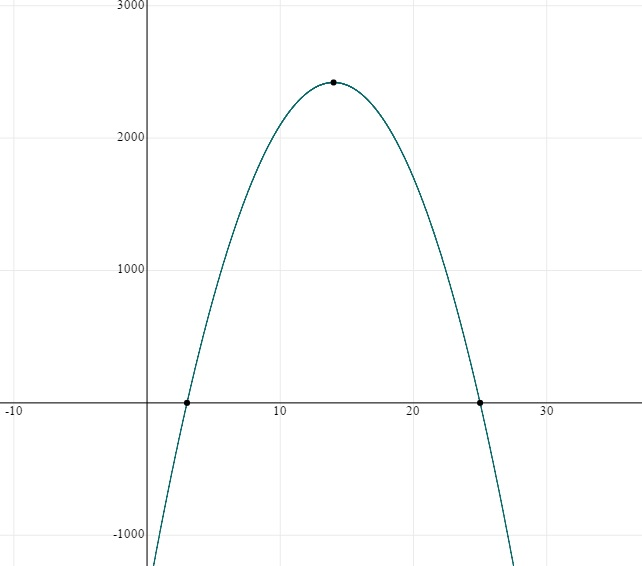
\includegraphics[width=15cm]{trojka.jpg}
	\end{center}
	\newpage
	
	\section*{5. príklad}
	Najděte největší a nejmenší hodnotu funkce $f(x)=(x+1)^{\frac{2}{3}}(2x-1)^3$ na intervalu <-1,1>.
	\begin{center}
		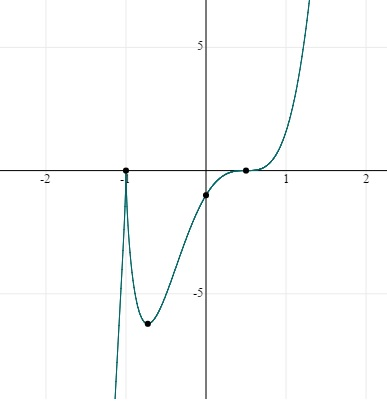
\includegraphics[width=10cm]{petka.jpg}
	\end{center}
	
	\begin{center}
	Funkciu zderivujeme, aby sme našli stacionárne body, ktoré môžu byť hľadaným minimom resp. maximom. Stacionárne body, sú body, v ktorých sa derivácia rovná 0. Stacionárny bod, v ktorom bude derivácia meniť svoje znamienko je aj lokálnym extrémom.
	\end{center}
	$$f(x)=(x+1)^{\frac{2}{3}}(2x-1)^3$$  
	$$f'(x)=\frac{2}{3}(x+1)^{-\frac{1}{3}}(2x-1)^3 + (x+1)^{\frac{2}{3}} \times 3(2x-1)^2 \times 2$$
	$$f'(x)=\frac{2(2x-1)^3}{3\sqrt[3]{x+1}} +6\sqrt[3]{(x+1)^2}(2x-1)^2 $$
	$$f'(x)=\frac{2(2x-1)^3}{3\sqrt[3]{x+1}} + \frac{6\sqrt[3]{(x+1)^2}(2x-1)^2 }{1} \times \frac{3\sqrt[3]{x+1}}{3\sqrt[3]{x+1}}$$
	$$f'(x)=\frac{2(2x-1)^3 + 18(x+1)(2x-1)^2}{3\sqrt[3]{x+1}}$$
	$$f'(x)=\frac{(2x-1)^2(2(2x-1) +18(x+1))}{3\sqrt[3]{x+1}}$$
	$$f'(x)=\frac{(2x-1)^2(4x-2+18x+18)}{3\sqrt[3]{x+1}}$$
	$$f'(x)=\frac{(2x-1)^2(22x+16)}{3\sqrt[3]{x+1}}$$
	$$\frac{(2x-1)^2(22x+16)}{3\sqrt[3]{x+1}}
	\Rightarrow
	x_{1}=\frac{1}{2}, x_{2}=-\frac{8}{11} $$
	\begin{center}	
	Stacionárne body a hranice intervalu následne dosadíme do pôvodnej funkcie a zistíme, v akom bode sa nachádza hľadané maximum a minimum.
	\end{center}
	
	$$f(-1) = 0$$
	$$f(-\frac{8}{11}) \doteq -6.2192$$ 
	$$f(\frac{1}{2})=0$$
	$$f(1)=\sqrt[3]{4}$$\\
	
	\begin{align*}
	\text{Lokálne minimum : } & f(-\frac{8}{11}) \doteq -6.2192\\
	\text{Lokálne maximum : } & f(1)=\sqrt[3]{4}
	\end{align*}
	
	
\end{document}